\cappar Nesta ocasião, tivemos a oportunidade que e funcionário da
Saema, Luis Arantes Lemos de Azevedo, nos visite em Espanha, e tivemos
e prazer de conversar com ele. Vamos contar algumas das nossas
conversas, que desejamos compartilhar com todos vocês. Obrigado, Luís,
pela tua visita!  \vspace{2cm}

{\bf Luís, fala-nos das tuas origens.}


\vspace{10pt}

Nasci em Luanda. O meu pai é da região de Bengo, e a minha mãe de
Luanda. Conheceram-se em Luanda e casaram. Da sua união nasceram 7
filhos, cinco meninas e dois meninos. Somos uma família muito unida, e
embora já cada um tenha a sua vida, todos os fins de semana fazemos
tudo por nos vermos e compartilhar.

\vspace{10pt}

{\bf Como viveu a guerra civil no seu país?}

\vspace{10pt}

Eu vivi em Luanda durante esses anos, e lá a guerra não foi tão
brutal, mas com certeza foi duro ver como as pessoas do meu país se
desmoronam e se afundam na destruição. Felizmente, agora o país está a
crescer e o espírito das pessoas é o de auto-superação e crescimento
constante, a formarem-se sempre que têm oportunidade para poderem
“subir na vida”.

\vspace{10pt}

{\bf Sobre a sua formação, Luis, pode resumi-la?}

\vspace{10pt}

Com certeza. Eu estudei no Instituto Médio Industrial de Luanda, na
especialização de Química. Depois disso vivi uma bela experiência a
trabalhar no ensino. Fui professor de escola durante alguns anos e
adorei ver que o que se ensina, serve para outros. Foi muito
gratificante. Depois, comecei a trabalhar na Saema, e já são 8 anos a
colaborar com eles. Na Saema, dedico-me à gestão administrativa,
controlo de salários, controlo de horários entre outras
coisas. Primeiro comecei a trabalhar em Cuanza Norte e depois de três
anos fui até Luanda, onde estou atualmente.

\vspace{10pt}

{\bf Como vê o trabalho que faz a Saema?}

\vspace{10pt}

Muito frutífero. O meu país está em crescimento, e são muitos os
lugares que se encontram sem água, sem luz, sem serviços médicos. A
Saema põe mais um grão de areia para realizar mudanças que as
autoridades vão conseguindo a pouco e pouco, e para que cada angolano
possa aceder aos serviços mínimos: luz, água e medicina. Apesar de
todas as dificuldades que tem o angolano, é uma pessoa que se esforça,
que trabalha e que deseja alegremente um futuro melhor.

\vspace{10pt}

{\bf Gosta de viajar?}

\vspace{10pt}

Sim. Antes de fazer esta viagem a Espanha, tinha viajado a países
perto de Angola. Esta é a minha primeira experiência na Europa. Adoro
viajar porque adoro ver como cada pessoa tem uma perceção do mundo,
como cada pessoa tem experiências distintas de trabalho, ver
diferentes ambientes. Todas as experiências me fazem ser uma pessoa
mais aberta. Gosto muito de viajar.

\vspace{10pt}

{\bf Qual é o seu autor favorito?}

\vspace{10pt}

Uanhenga Xitu, ele marcou-me desde a minha adolescência e é um referente para mim.

\vspace{10pt}

{\bf Pedimos sempre aos nossos entrevistados que enviem uma mensagem
  ao seu povo. Que mensagem envia, Luís?}

\vspace{10pt}

Tenham esperança, o futuro vai ser melhor. 


\vspace{10pt}

{\bf Obrigado, Luís. Desejamos-lhe o melhor, e desejamos-lhe um feliz casamento, visto que vai casar em breve. Felicidades e, \textcolor{red}{vivam os noivos!}}

  \begin{figurebox}
    \vspace{20pt}
    \centering
    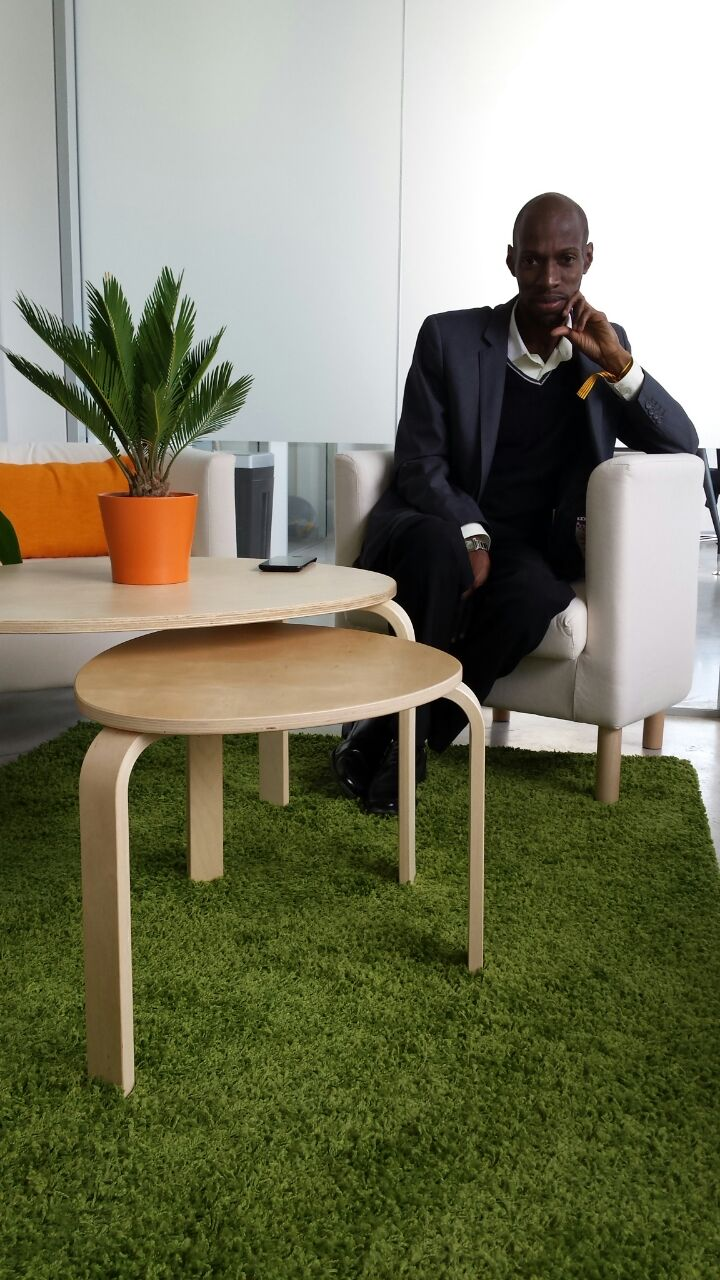
\includegraphics[scale=0.3]{luis.jpg}

     Luis Arantes Lemos de Azevedo\\
    {\sl Coordenador administração do Saema}
    \vspace{20pt}
  \end{figurebox}

\newpage

%%% Local Variables: 
%%% mode: latex
%%% TeX-master: "solucionenaccion"
%%% End: 



